In this section, we define new terms that represent {\it multi-order ego networks} and {\it multi-order
friendship networks}, and then present several properties of the multi-order friendship networks.
Our betweenness computation algorithm in Section~\ref{sec:betweenness} takes advantage of these properties.
\begin{table}[t]
\center
\caption{Summary of notation}\label{table:symbols}
\small
    \begin{tabular}{| p{1.2cm} | p{10cm} |}
        \hline
        Symbol & Description \\
        \hline
        \hline
        $\V{v}{i}$ & set of $i$-hop neighbors of vertex $v$ ($\V{v}{0} = \{ v \}$)\\
        $\LV{v}{i}$ & set of vertices that are at most $i$ hops away from vertex $v$ (i.e., $\LV{v}{i} = \cup_{k = 0}^{i} \V{v}{k}) $\\
        $\E{v}{i}$ & set of edges connecting two vertices in $\V{v}{i}$ ($\E{v}{0}$=$\emptyset$)\\
        $\LE{v}{i}$ & set of edges connecting two vertices in $\LV{v}{i}$\\
        \hline
    \end{tabular}
\end{table}

%\begin{figure}[t]
%        \captionsetup[subfigure]{aboveskip=-1pt,belowskip=-1pt}
%        \centering
%        \begin{subfigure}[b]{0.7\textwidth}
%                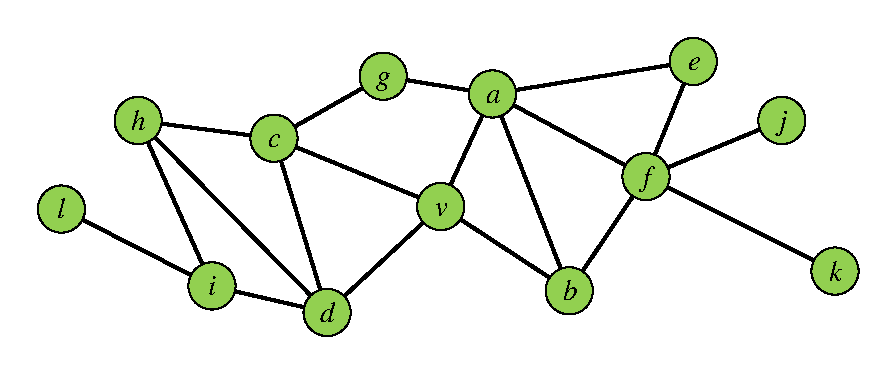
\includegraphics[width=\textwidth]{./images/figs-original.pdf}
%                \caption{A given network}
%                \label{fig:1-a}
%        \end{subfigure}
%
%        \begin{subfigure}[b]{0.3\textwidth}
%                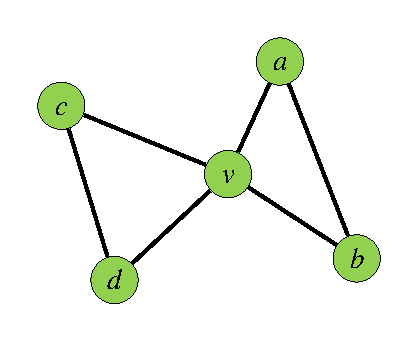
\includegraphics[width=\textwidth]{./images/ego2.pdf}
%                \caption{Ego network, $\ENN{v}{1}$}
%                \label{fig:1-b}
%        \end{subfigure}
%        \begin{subfigure}[b]{0.5\textwidth}
%                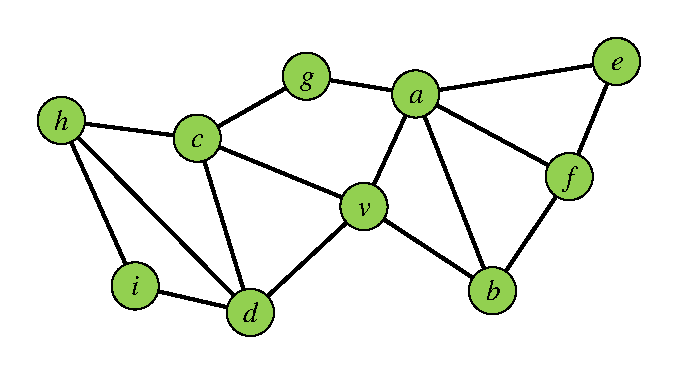
\includegraphics[width=\textwidth]{./images/second-order.pdf}
%                \caption{Second-order ego network, $\ENN{v}{2}$}
%                \label{fig:1-c}
%        \end{subfigure}
%
%        \begin{subfigure}[b]{0.3\textwidth}
%                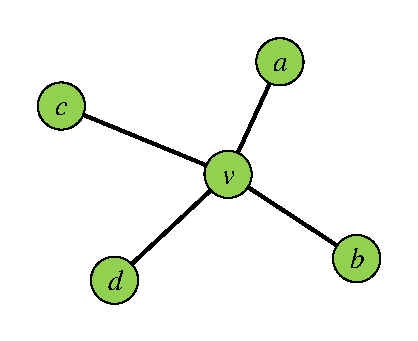
\includegraphics[width=\textwidth]{./images/friends.pdf}
%                \caption{Friendship network, $\ENN{v}{1}$}
%                \label{fig:1-d}
%        \end{subfigure}
%        \begin{subfigure}[b]{0.5\textwidth}
%                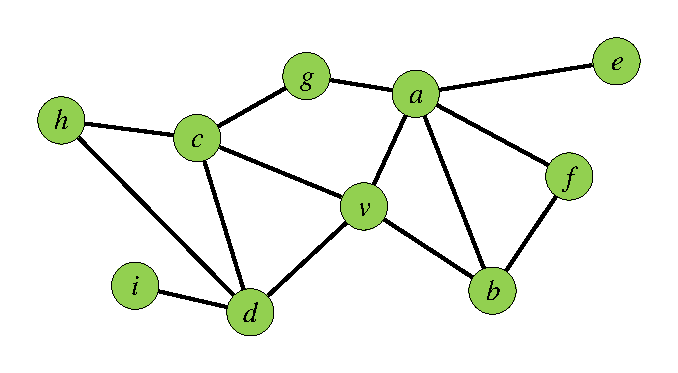
\includegraphics[width=\textwidth]{./images/multi-oder-friends.pdf}
%                \caption{Second-order friendship network, $\ENN{v}{2}$}
%                \label{fig:1-e}
%        \end{subfigure}
%
%        \caption{The given network, and the multi-order ego and friendship networks of vertex $v$}
%        \label{fig:1}
%\end{figure}
%
%\begin{figure}[t]
%    \captionsetup[subfigure]{aboveskip=0pt}
%    \centering
%    \subfigure[A given network]{
%        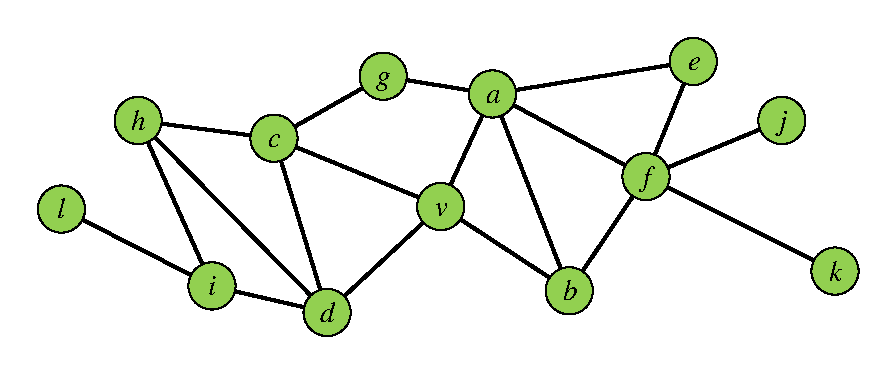
\includegraphics[width=0.65\linewidth]{./images/figs-original.pdf}
%    }\label{original}\vspace*{-0.1cm}
%
%    \subfigure[Ego network, $\ENN{v}{1}$]{
%        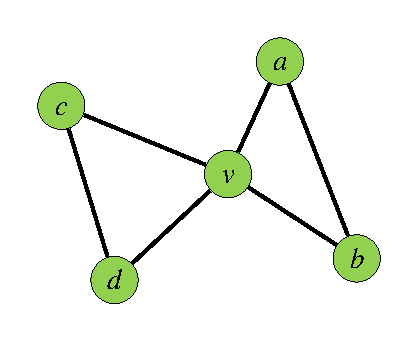
\includegraphics[width=0.3\linewidth]{./images/ego2.pdf}
%    }\label{eego_b}\vspace*{-0.1cm}
%    \subfigure[Second-order ego network, $\ENN{v}{2}$]{
%        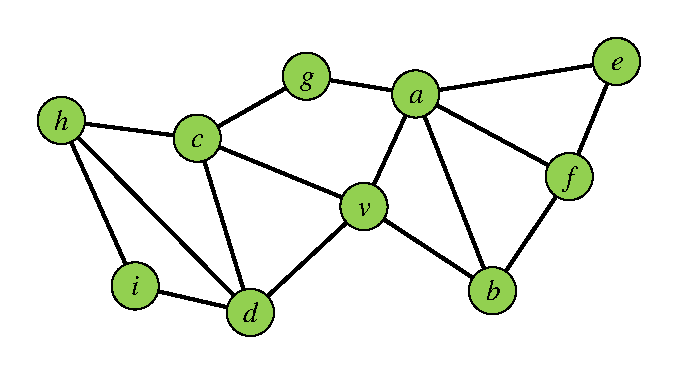
\includegraphics[width=0.45\linewidth]{./images/second-order.pdf}
%    }\label{soego}\vspace*{-0.1cm}
%
%    \subfigure[Friendship network, ]{
%        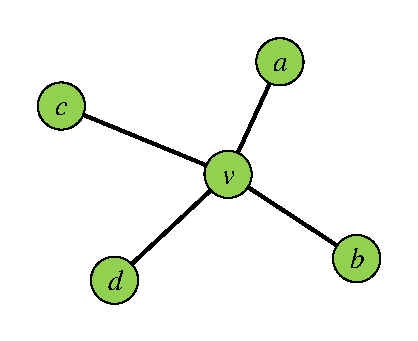
\includegraphics[width=0.3\linewidth]{./images/friends.pdf}
%    }\label{eego_f}
%    \subfigure[Second-order friendship network, $\XN{v}$]{
%        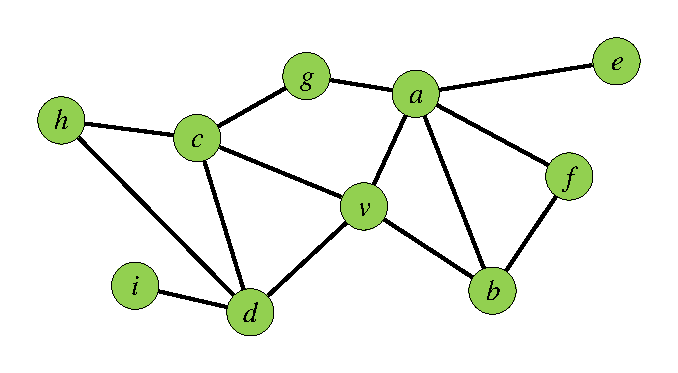
\includegraphics[width=0.45\linewidth]{./images/multi-oder-friends.pdf}
%    }\label{eego_c}
%    \caption{The ego, multi-order, and multi-layered ego networks of vertex $v$}
%    \label{eego2}
%\end{figure}

\subsection{Definitions}\label{subsec:x-egoDefinition}
In this paper, we consider a graph $G(V, E)$\footnote{We use the term {\em actors} and {\em social links} to refer to individuals, groups or organizations and their relationships in a social network. On the other hand, the graph representing a social network consists of {\em vertices} and {\em edges} representing actors and social links, respectively.}
where $V$ is a set of vertices and $E$ is a set of undirected edges representing social links between vertices.
In the literature~\cite{egocentric, everett, ICCN:lbcdna, SIMBET}, given a graph $G(V, E)$ and a vertex $v \in V$, the {\em ego network} of $v$ is defined as the subgraph of $G$ consisting of $v$ and its 1-hop neighbors (i.e., vertices with an edge to $v$) as well as the edges between these vertices.
Using the notation summarized in Table~\ref{table:symbols}, this ego network can be formally extended as
follows:
\begin{definition}\label{def:multi-order-ego-network}
Given a graph $G(V, E)$ and a vertex $v \in V$, the \emph{multi-order ego network} of $v$ is defined as $\ENN{v}{n}
(\LV{v}{n}, \LE{v}{n})$ where $\LV{v}{n}$ is the set of vertices whose shortest distance from $v$ is no longer than $n$ (i.e., $\{ v \} \sum \V{v}{n}$) and $\LE{v}{n}$ denotes the set of edges between the vertices in $\LV{v}{n}$.
\end{definition}
In a given graph shown at Fig.~\ref{eego2} (a), $\LV{v}{1} = \V{v}{0} \cup \V{v}{1} = \{v, a, b, c, d\}$ and $\LE{v}{1}=\{ \{v, a\}, \{v, b\}, \{v, c\}, \{v, d\},$ $\{a, b\}, \{c, d\} \}$.
The ego network of vertex $v$, $\EN{v}(\LV{v}{1}, \LE{v}{1})$, is shown in Fig.~\ref{eego2} (b).
Ego networks well model the relationships/interactions between an actor and others in a social network.
However, ego networks have the limitation that it does not capture a substantial amount of information.
For example, in Fig.~\ref{eego2} (a), assume that actor $v$ received from actor $a$ the information about $a$'s 1-hop neighbors (i.e., $b$, $e$, $f$, $g$, and $v$).
Despite this information, the ego network of $v$ cannot record the social links between $a$ and $e$, between $a$ and $f$, and between $a$ and $g$ since it can represent only the social links between $v$ and each 1-hop neighbor of $v$, and between two 1-hop neighbors of $v$.
On the other hand, {\it multi-order ego networks}, defined as $\ENN{v}{n} (\LV{v}{n}, \LE{v}{n})$, can hold more
information than ego networks. The second-order ego network of vertex $v$, $\ENN{v}{2} (\LV{v}{2}, \LE{v}{2})$, is shown
in Fig.~\ref{eego2} (c).

To overcome the above limitation, we introduce the following extension to ego networks:
\begin{definition}\label{def:multi-order-network}
Given a graph $G(V, E)$ and a vertex $v \in V$, the \emph{n-order ego network} of $v$ is $\ENN{v}{n}(\LV{v}{n}, \LE{v}{n} - \E{v}{n})$, where $\LV{v}{n}$ is the set of vertices that are at most $n$ hops away from $v$, $\LE{v}{n}$ is the set of edges between vertices that are at most $n$ hops away from $v$, and $\E{v}{n}$ is the set of edges between $n$-hop neighbors of $v$.
\end{definition}
Fig.~\ref{eego2} (c) shows the 2-laye{subsec:x-egoDefinition} $v$. The 2-layered ego network is different from 2nd order ego networks of which edge sets includes $\E{v}{n}$.
It means that a vertex $v$ can generate its x-ego network by using the neighbor information of its neighbors. In summary, both ego and x-ego networks can be obtained with the same (similar) network overhead.
% However, expanded ego networks inherently contain substantially larger amounts of information than ego networks.
% As experimentally demonstrated in Section~\ref{experiments}, highly accurate betweenness centrality values can be obtained from x-ego networks than ego networks.
Fig.~\ref{eego2}(b) shows the x-ego network of $v$ from the graph in Fig.~\ref{eego}.
As Fig.~\ref{eego2}(a) and Fig.~\ref{eego2}(b) illustrate, the x-ego network of $v$ is different from the ego network of $v$ in that {subsec:x-egoDefinition}neighbors of $v$ (i.e., $\LV{v}{2} - \LV{v}{1} = \V{v}{2}$) as well as the edges between a 1-hop neighbor and a 2-hop neighbor of $v$.
Despite th{subsec:x-egoDefinition}h the ego and x-ego networks of $v$ can be obtained with the same network overhead (since they consume the same messages from 1-hop neighbors of $v$).
The benefits of x-ego networks over ego networks are further verified in Section~\ref{evaluation}.
% For a given graph $G(V, E)$ a{subsec:x-egoDefinition}rtex $v$, we define the following terms:
% \begin{itemize}
% \item $V_{i}^{v}$: the set of vertices whose shortest distance from $v$ is no larger than $i$ (hence, $V_{0}^{v}=\{v\}$).
% \item $E_{i}^{v}$: the set of edges on shortest paths from $v$ to a node in $V_{i}^{v}$ (hence, $E_{0}^{v}=\emptyset$).
% \item $E_{i \mhyphen j}^{v}$: the set of edges between an $i$-hop neighbor and a $j$-hop neighbor of $v$ (hence, $E_{0 \mhyphen 0}^{v}=\e{subsec:x-egoDefinition} $N_{i}$: the set of 1-hop neighbor nodes with a direct link to $v_i$.
% \item $E_{i}$: the set of links between $v_i$ to the nodes in $N_{i}$.
% \item $\bar{E}_{i}$: the set of links among the nodes in $N_{i}$.
% \end{itemize} 
%The ego network model has been frequently used in many network analysis. The ego network is the network consisting of a single node(ego) together with the 1st-hop neighbor nodes they are connected to and all the li{subsec:x-egoDefinition}ighbors.
% We also define the following additional terms:
% \begin{itemize}
% \item $N^{2}_{i}$: the set of $v_i$'s 2-hop neighbor nodes each of which has a direct link to a node in $N_{i}$.
% \item $E^{2}_{i}$: the set of links connecting the $N_{i}$ nodes to the $N^{2}_{i}$ nodes.
% %\item $\ddot{E}_{N^{2}_{i}}$: the set of edges of nodes belong to $N^{2}_{i}$.
% \end{itemize}